\chapter{Evolution of system design}
\label{chap:evolution}

To track sleep unobtrusively, multiple techniques and sensor types have been tested and evaluated by other researchers. Piezoelectric film sensor were placed on a rodent cage and signals were used for recognition of breathing and movement\cite{piezo}. In same way, sleep and awakening was recorded in humans using load cells placed under bed supports\cite{load_cells}. Subjects were also recorded using infrared cameras and this method provided 19\% better recognition of small movements than actigraphy done with a wrist worn device\cite{video}. \ac{POF} sensors were also used to recognize breathing patterns and detect apnea\cite{optical}. In another research, a group of researchers conducted experiment in which they placed two 24\ac{GHz} radars under the bed in a nursing home and found out that it is possible to accurately recognize the hearth rate\cite{radar}. Using pressure sensitive e-textile it is possible to classify a sleep stage as awake, \ac{NREM} or \ac{REM}\cite{e-textile}. And using pneumatic pressure sensors placed in a sealed air-cushion that is placed under the bed it is possible to measure hearth beat, respiration, snoring and movement\cite{pneumatic}.

\section{Devices and technology}

Current setup is based on work of Prof. Dr. Ralf Seepold, Ra\'ina Kuhn, Daniel Scherz and Maxime Guyot at \ac{UC-Lab}\cite{Kuhn}\cite{Guyot}. 

\begin{figure}[h]
  \begin{center}
    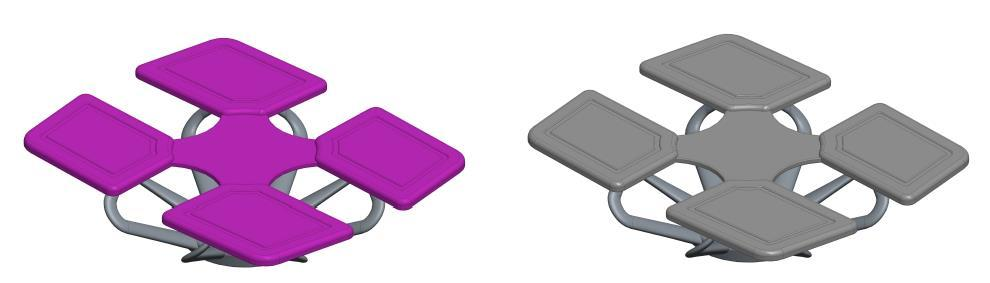
\includegraphics[width=0.6\linewidth]{1-base_plate.jpg}
  \end{center}
  \caption{Base plates in the bed.}
  \label{fig:base-plate}
\end{figure}

\begin{figure}[h]
  \begin{center}
    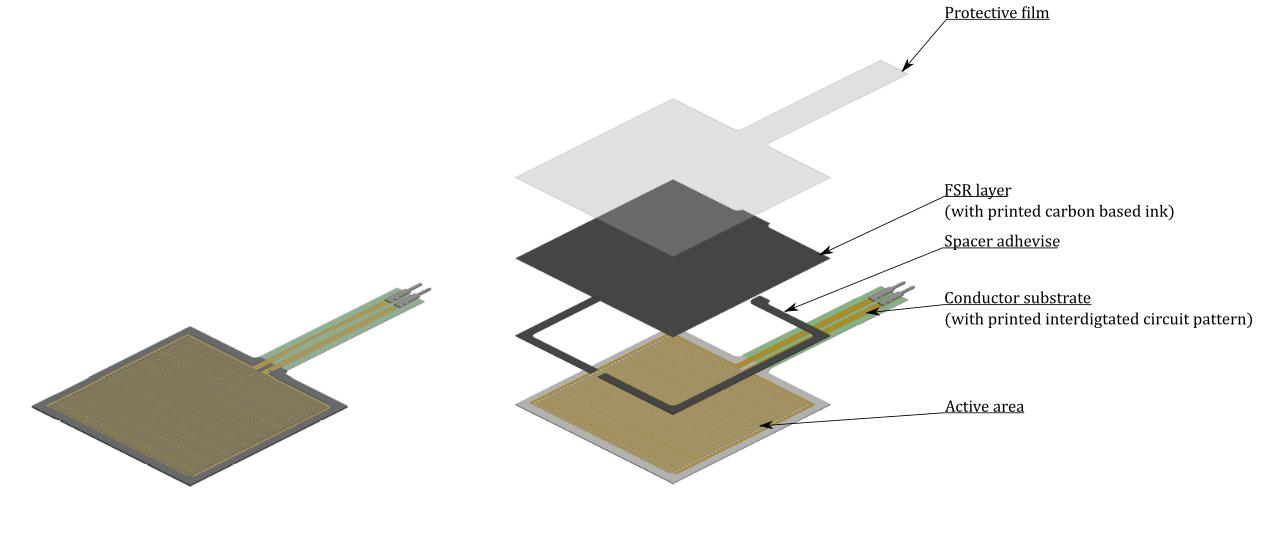
\includegraphics[width=0.7\linewidth]{1-fsr_sensor.png}
  \end{center}
  \caption{Layout of sensors in a bed.}
  \label{fig:fsr-sensor}
\end{figure}


\section{Test environment}

\begin{figure}[h]
  \begin{center}
    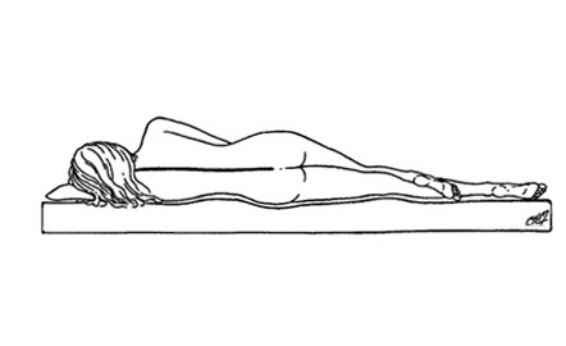
\includegraphics[width=0.4\linewidth]{1-weight_distribution.png}
    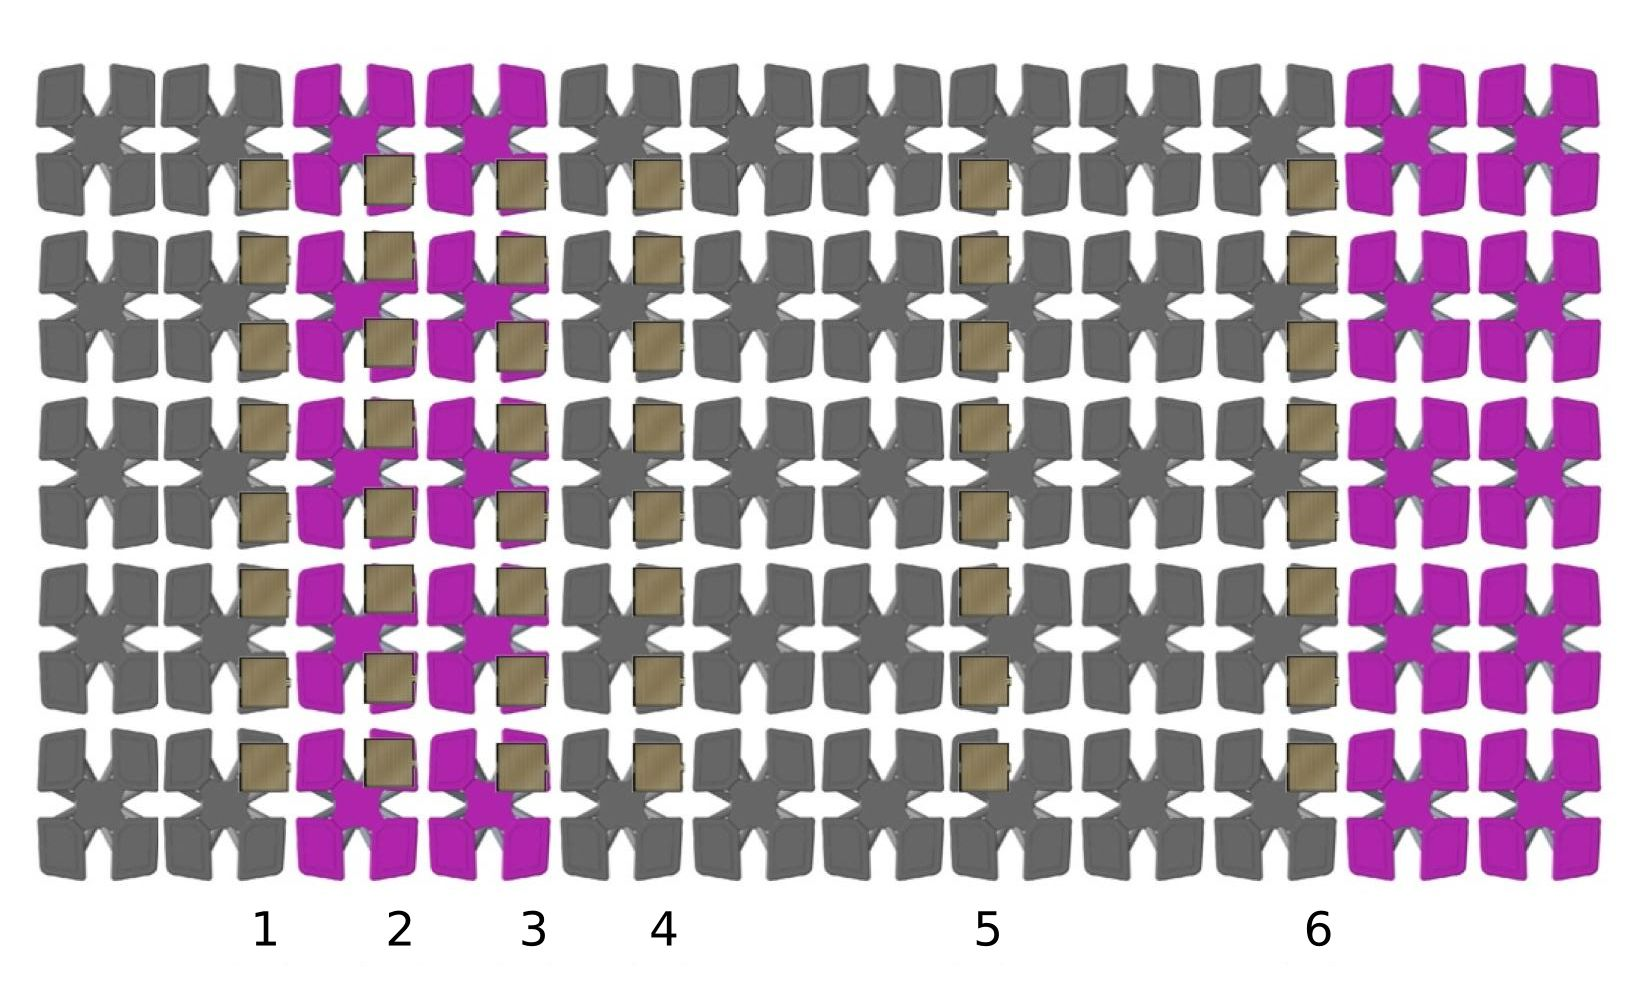
\includegraphics[width=0.4\linewidth]{1-sensor_layout.jpg}
  \end{center}
  \caption{Sensor arrangement in bed compared to sleep position.}
  \label{fig:sensor-layout}
\end{figure}

\begin{figure}[h]
  \begin{center}
    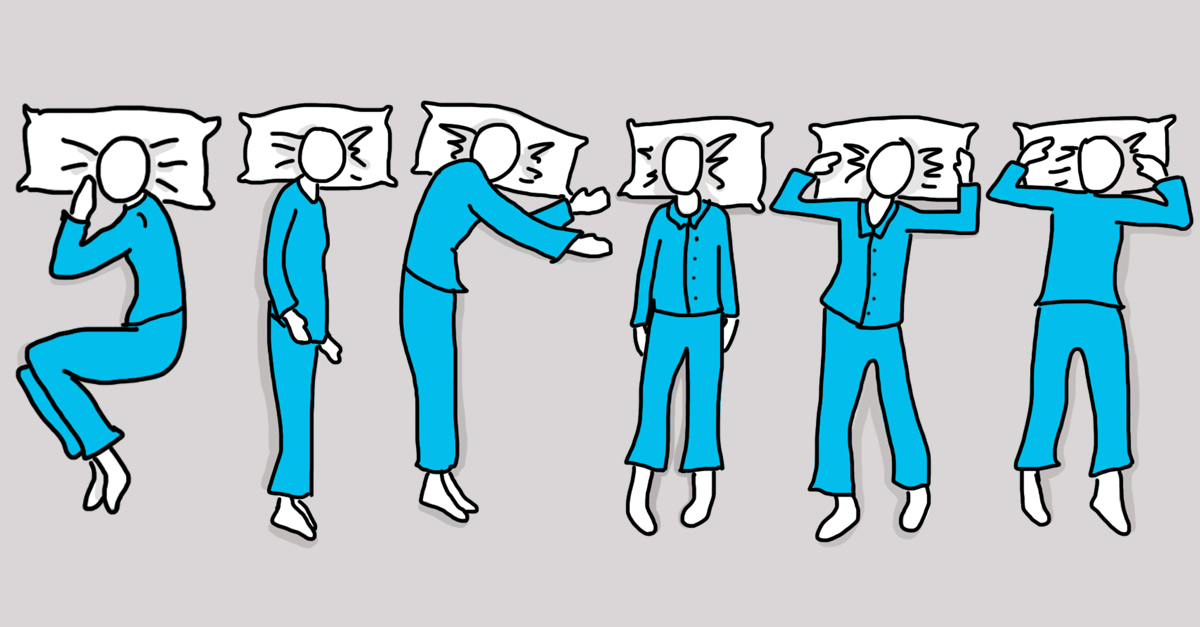
\includegraphics[width=0.4\linewidth]{1-sleep_positions.jpg}
  \end{center}
  \caption{Different sleep positions.}
  \label{fig:sleep_positions}
\end{figure}


\section{Results so far}


